% Author: Izaak Neutelings (Februari, 2020)
% http://texample.net/tikz/examples/tag/circuitikz/
% http://texample.net/tikz/examples/circuitikz/
% https://www.overleaf.com/learn/latex/CircuiTikz_package
% http://texdoc.net/texmf-dist/doc/latex/circuitikz/circuitikzmanual.pdf
% http://repositorios.cpai.unb.br/ctan/graphics/pgf/contrib/circuitikz/circuitikzmanual.pdf
\documentclass[border=3pt,tikz]{standalone}
\usepackage{amsmath} % for \dfrac
\usepackage{physics}
\usepackage{tikz,pgfplots}
\usepackage[siunitx]{circuitikz} %[symbols]
\usepackage[outline]{contour} % glow around text
\usetikzlibrary{arrows,arrows.meta}
\usetikzlibrary{decorations.markings}
\tikzset{>=latex} % for LaTeX arrow head
\usepackage{xcolor}
\colorlet{Icol}{blue!50!black}
\colorlet{Ccol}{orange!90!black}
\colorlet{Rcol}{green!50!black}
\colorlet{Lcol}{violet!90}
\colorlet{loopcol}{red!90!black!25}
\colorlet{pluscol}{red!60!black}
\colorlet{minuscol}{blue!60!black}
\newcommand\EMF{\mathcal{E}} %\varepsilon}
\contourlength{1.5pt}
\tikzstyle{EMF}=[battery1,l=$\EMF_0$,invert]
\tikzstyle{internal R}=[R,color=Rcol,Rcol,l=$r$,/tikz/circuitikz/bipoles/length=30pt]
\tikzstyle{loop}=[->,red!90!black!25]
\tikzstyle{loop label}=[loopcol,fill=white,scale=0.8,inner sep=1]
\tikzstyle{thick R}=[R,color=Rcol,thick,Rcol,l=$R$]
\tikzstyle{thick C}=[C,thick,color=Ccol,Ccol,l=$C$]
\tikzstyle{thick L}=[L,thick,color=Lcol,Lcol,l=$L$,/tikz/circuitikz/bipoles/length=56pt] %inductor
\tikzstyle{myswitch}=[closing switch,line width=0.3] %-{Latex[length=3]}
\newcommand{\closedswitch}[1]{
  \draw[line width=0.6] (#1) --++ (0.48,0);
  \fill[black] (#1) circle (0.03);
}


\newcommand{\myvoltmeter}[2] 
{  % #1 = name , #2 = rotation angle
  \begin{scope}[transform shape,rotate=#2]
  \draw[thick] (#1)node(){$\mathbf V$} circle (11pt);
  \draw[rotate=45,-latex] (#1)  +(-17pt,0) --+(17pt,0);
  \end{scope}
}



\begin{document}


% R with CLOSED switch
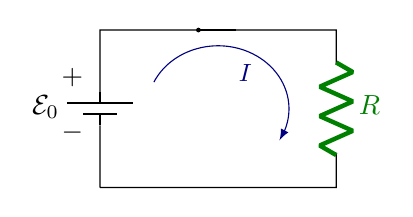
\begin{tikzpicture}
  \def\ang{155}
  \def\a{0.9}
  \def\b{0.8}
  \draw[->,Icol] ({1.5+\a*cos(\ang)},{1+\b*sin(\ang)}) arc (\ang:-30:{\a} and {\b})
                 node[midway,left=2,below=1,scale=0.9] {$I$};
  \draw (0,0) to[EMF] (0,2) --++(3,0)
              to[thick R] ++(0,-2) -- (0,0);
  \closedswitch{1.25,2};
  \node at (-0.35,0.7) {$-$};
  \node at (-0.35,1.4) {$+$};
\end{tikzpicture}


% RL with CLOSED switch
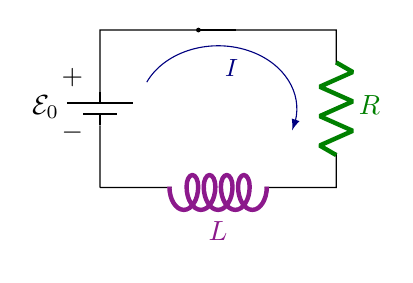
\begin{tikzpicture}
  \def\ang{155}
  \def\a{1.0}
  \def\b{0.8}
  \draw (0,0) to[EMF] (0,2) --++(3,0) %to[myswitch]
              to[thick R] ++(0,-2) to[thick L] (0,0);
  \draw[->,Icol] ({1.5+\a*cos(\ang)},{1+\b*sin(\ang)}) arc (\ang:-20:{\a} and {\b})
                 node[midway,left=6,below=0,scale=0.9] {$I$};
  \closedswitch{1.25,2};
  \node at (-0.35,0.7) {$-$};
  \node at (-0.35,1.4) {$+$};
  %\node at ( 0.90,0.34) {$-$};
  %\node at ( 2.10,0.34) {$+$};
  %\node at ( 1.50,0.39) {$\EMF$};
\end{tikzpicture}


% RC with OPEN switch
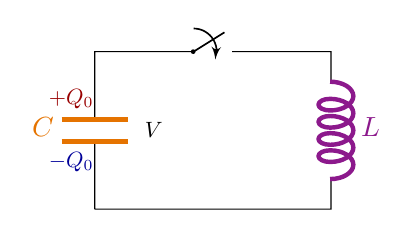
\begin{tikzpicture}
  \def\ang{120}
  \def\a{1.0}
  \def\b{0.8}
  \draw (0,0) to[thick C] (0,2) to[myswitch] ++(3,0)
              to[thick L] ++(0,-2) -- (0,0);
  \fill[black] (1.25,2) circle (0.03);
  \node[minuscol,scale=0.8] at (-0.3,0.6) {$-Q_0$};
  \node[pluscol,scale=0.8] at (-0.3,1.4) {$+Q_0$};
  \node[scale=0.8] at (0.75,1) {$V$};
\end{tikzpicture}


% RCL with OPEN switch
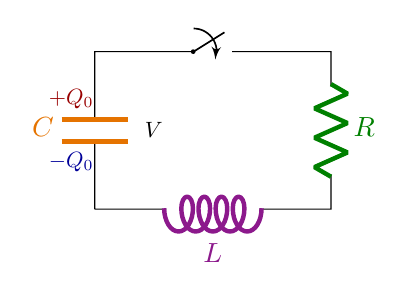
\begin{tikzpicture}
  \def\ang{120}
  \def\a{1.0}
  \def\b{0.8}
  \draw (0,0) to[thick C] (0,2) to[myswitch] ++(3,0)
              to[thick R] ++(0,-2) to[thick L] (0,0);
  \fill[black] (1.25,2) circle (0.03);
  \node[minuscol,scale=0.8] at (-0.3,0.6) {$-Q_0$};
  \node[pluscol,scale=0.8] at (-0.3,1.4) {$+Q_0$};
  \node[scale=0.8] at (0.75,1) {$V$};
\end{tikzpicture}


\end{document}
